\documentclass[letterpaper]{article}

\usepackage{aaai}
\usepackage{times}
\usepackage{helvet}
\usepackage{courier}
\usepackage[pdftex,dvipsnames]{xcolor}
\usepackage{xargs}
\usepackage{hyperref}
\usepackage{listings}
\usepackage{multicol}

\usepackage[colorinlistoftodos,prependcaption,textsize=tiny]{todonotes}
\newcommandx{\unsure}[2][1=]{\todo[linecolor=red,backgroundcolor=red!25,textcolor=black,bordercolor=red,#1]{#2}}
\newcommandx{\change}[2][1=]{\todo[linecolor=blue,backgroundcolor=blue!25,bordercolor=blue,#1]{#2}}
\newcommandx{\info}[2][1=]{\todo[linecolor=OliveGreen,backgroundcolor=OliveGreen!25,bordercolor=OliveGreen,#1]{#2}}
\newcommandx{\improvement}[2][1=]{\todo[linecolor=Plum,backgroundcolor=Plum!25,bordercolor=Plum,#1]{#2}}
\newcommandx{\thiswillnotshow}[2][1=]{\todo[disable,#1]{#2}}

\frenchspacing
\setlength{\pdfpagewidth}{8.5in}
\setlength{\pdfpageheight}{11in}
\pdfinfo{
/Title (Finding Parallel Regions with Temporal Planning)
/Author (Claudio Scheer)}
\setcounter{secnumdepth}{0}

\lstdefinestyle{pddlStyle}{
    captionpos=b,
    numbers=left,
    numberstyle=\tiny,
    numbersep=6pt,
    % language=Lisp,
    % xleftmargin=12pt,
    stringstyle=\ttfamily\small,
    basicstyle=\ttfamily\tiny,
    showstringspaces=false,
    breaklines,
    frame=single,
    escapechar=|,
    keywords={
        % at,
        % start,
        % end,
        % forall
    },
    otherkeywords={
        :duration,
        :durative-action,
        :parameters,
        :condition,
        :effect,
        :goal,
        :init
    },
    columns=fullflexible,
}

\lstdefinestyle{cppStyle}{
    captionpos=b,
    numbers=left,
    numberstyle=\tiny,
    numbersep=6pt,
    language=c++,
    % xleftmargin=12pt,
    stringstyle=\ttfamily\small,
    basicstyle=\ttfamily\tiny,
    showstringspaces=false,
    breaklines,
    frame=single,
    escapechar=|,
    columns=fullflexible,
}


\begin{document}

\title{Finding Parallel Regions with Temporal Planning}
\author{Claudio Scheer\\
    Master's Degree in Computer Science\\
    Pontifical Catholic University of Rio Grande do Sul - PUCRS\\
    Porto Alegre - RS, Brazil\\
    claudio.scheer@edu.pucrs.br\\
}
\maketitle

\begin{abstract}
    \begin{quote}
        Abstract.
    \end{quote}
\end{abstract}

\noindent Introduction.


\section{Bibliography}

\subsection{Temporal Plannign} \label{label:temporal-planning}

According to \cite{DBLP:series/synthesis/2019Haslum}, actions in temporal planning have a duration. Therefore, the planner will try to find a schedule in which some actions can be executed in parallel.

There are different approaches that can be used to formalize temporal actions with PDDL. In this paper, I used \texttt{:durative-action}. This action is represented in four sections, as listed below.

\begin{itemize}
    \item \texttt{:parameters}: parameters needed to execute the action;
    \item \texttt{:duration}: time the action takes to run;
    \item \texttt{:condition}: conditions that need to be respected to apply the effects;
    \item \texttt{:effect}: effects that will be applied to the state;
\end{itemize}

The sections \texttt{:condition} and \texttt{:effect} are separated in three categories: \texttt{at start}, \texttt{over all} and \texttt{at end}. As described by \cite{DBLP:series/synthesis/2019Haslum}, these categories represent the conditions and effects used at each stage of the action. The \texttt{at start} statements are used when starting the action. The \texttt{over all} statements are used during the time the action is being executed. The \texttt{at end} statements are used at the end of the action.

\improvement[inline]{The following section may not be necessary.}
I must mention that \texttt{:durative-action} can be translated into instantaneous actions. Here is the paper: \cite{DBLP:conf/ecai/ScalaHTR16}.


\subsection{STP}

I used the STP (Simultaneous Temporal Planner) planner, introduced by \cite{Blanco2018ForwardsearchTP}, to find the best temporal plan. STP uses a modified version of the Fast Downward \cite{Helmert_2006} planner that can generate a temporal plan. The version used in this paper is provided by the Artificial Intelligence and Machine Learning Group - Universitat Pompeu Fabra\footnote{\href{https://github.com/aig-upf}{https://github.com/aig-upf}}.

The STP planner needs to receive as a parameter the maximum number of actions that can be executed at the same time. When finding parallel regions, this parameter is a problem, because we do not know how many instructions can be executed in parallel. Therefore, in some cases, it is necessary to test different values for this paramenter.
\info[inline]{The higher this number, the more time it takes to solve the problem.}


\section{Source Code Translation}

\info[inline]{Describe here some patterns on how to convert source code into the PDDL problem.}


\section{Formalization}

I used only two \texttt{:durative-action} to formalize the problem. One to handle assignment instructions and another to handle binary operations. Binary operations must be understood as any operations (sum, multiplication, XOR, etc) that involve two variables.

All \texttt{:durative-action} must have a duration time. However, since my objective is not to cover the execution time of the instructions in this paper, I set the duration time to 1 for all actions. This approach ensures that when operations cannot be executed in parallel, the total execution time will be increased by one. In a future work, it may be a good approach to define different duration time for each instruction.

\change[inline]{In a future work, it may be a good approach to define different duration time for each instruction.}

By definition, each operation and assignment instruction must have an identifier. With this identification, we can create the dependency tree for the instructions. The dependency tree makes it easy to test whether all dependencies for a specific instruction have already been executed. Since each problem has a specific dependency tree, the dependency tree must be defined in the initial state of the problem. In the initial state, in addition to the dependency tree, the identifier for the operation and assignment instructions must also be defined.

As discussed in Section Temporal Plannign, the sections \texttt{:conditions} and \texttt{:effects} have three different categories. In my formalization, all preconditions must be respected at the beginning of the action and the effects is applied only at the end of the action.

\subsection{Assignment action}

The assignment action will receive the assignment instruction and the instruction identifier as a parameter. The first two conditions will ensure that the identifier belongs to the the instruction and that the assignment has not yet been executed.

The third condition is common the all durative actions. The \texttt{forall} operator loops through all identifiers in the dependency tree, testing whether the identifier is parent of the current instruction and whether the parent instruction have already been executed.

The Table~\ref{table:forall-truth-table} shows the truth table that represents the condition within the \texttt{forall} operator. The variable $A$ represents that the current identifier is a child of the parent identifier. $B$ represents that the parent identifier has already been executed. As shown in the truth table, the only case where the condition returns false is when the current identifier is a child of the parent identifier and the instruction represented by the parent identifier has not yet been executed.

\begin{table}[h]
    \centering
    \begin{tabular}{|c|c|c|}
        \hline
        $A$ & $B$ & $\neg A \lor B$ \\
        \hline
        1   & 1   & 1               \\
        1   & 0   & 0               \\
        0   & 1   & 1               \\
        0   & 0   & 1               \\
        \hline
    \end{tabular}
    \caption{Dependency tree condition truth table}
    \label{table:forall-truth-table}
\end{table}

The \texttt{:effect} of the assignment action is to mark the instructions as executed. The Listing~\ref{lst:assignment-action} shows the formalization of the assignment action.

\begin{lstlisting}[caption=Formalization of the assignment action,label=lst:assignment-action,style=pddlStyle]
(:durative-action assignment
    :parameters (
        ?instruction_id - id
        ?id - assignment
    )
    :duration (= ?duration 1)
    :condition (and
        (at start (assignment_id ?id ?instruction_id))
        (at start (not (executed_assignment ?id)))
        (at start (forall (?parent - id)
            (or
                (not (dependency_tree ?parent ?instruction_id))
                (executed_instruction ?parent)
            )
        ))
    )
    :effect (and
        (at end (executed_instruction ?instruction_id))
        (at end (executed_assignment ?id))
    )
)
\end{lstlisting}

\subsection{Binary operation action}

This action is responsible for executing a binary operation between two variables. The action takes as parameters the two assignment variables that will be used in the operation and the assignment instruction that will receive the result of the binary operation.

Here, the conditions to execute the action are that the binary operation has not yet been executed and the assignment instructions of the two input variables have already been executed.

As shown in Listing~\ref{lst:binary-operation-action}, the effects are similar to the previous action: the binary operation is marked as executed, releasing the next instructions that holds in this operation.

\begin{lstlisting}[caption=Formalization of the binary operation action,label=lst:binary-operation-action,style=pddlStyle]
(:durative-action binary_operation
    :parameters (
        ?instruction_id - id
        ?idA - assignment
        ?idB - assignment
        ?operation_id - operation
        ?idC - assignment
    )
    :duration (= ?duration 1)
    :condition (and
        (at start (operation_id ?operation_id ?instruction_id))
        (at start (forall (?parent - id)
            (or
                (not (dependency_tree ?parent ?instruction_id))
                (executed_instruction ?parent)
            )
        ))
        (at start (not (executed_operation ?operation_id)))
        (at start (not (executed_binary_operation ?idA ?idB ?operation_id ?idC)))
        (at start (executed_assignment ?idA))
        (at start (executed_assignment ?idB))
    )
    :effect (and
        (at end (executed_instruction ?instruction_id))
        (at end (executed_operation ?operation_id))
        (at end (executed_binary_operation ?idA ?idB ?operation_id ?idC))
    )
)
\end{lstlisting}

\section{Results}

In this section, I will show a simple example of formalization. Regarding our objective, we hope that the temporal plan found by the planner shows the instructions that we can execute in parallel.

The example is represented by the source code shown in Listing~\ref{lst:source-code}. This simple source code sums two variables and set the result in the variable \texttt{c}. The variables \texttt{a} and \texttt{b} are not dependent on each other. Therefore, we must be able to execute the two assignment instructions in parallel, as shown in Figure~\ref{fig:dependency-tree-parallel}.

\begin{lstlisting}[caption=Source code,label=lst:source-code,style=cppStyle]
#include <iostream>

int main()
{
    int a = 3;
    int b = 3;
    int c = a + b;
    return 0;
}
\end{lstlisting}

\begin{figure}[h]
    \centering
    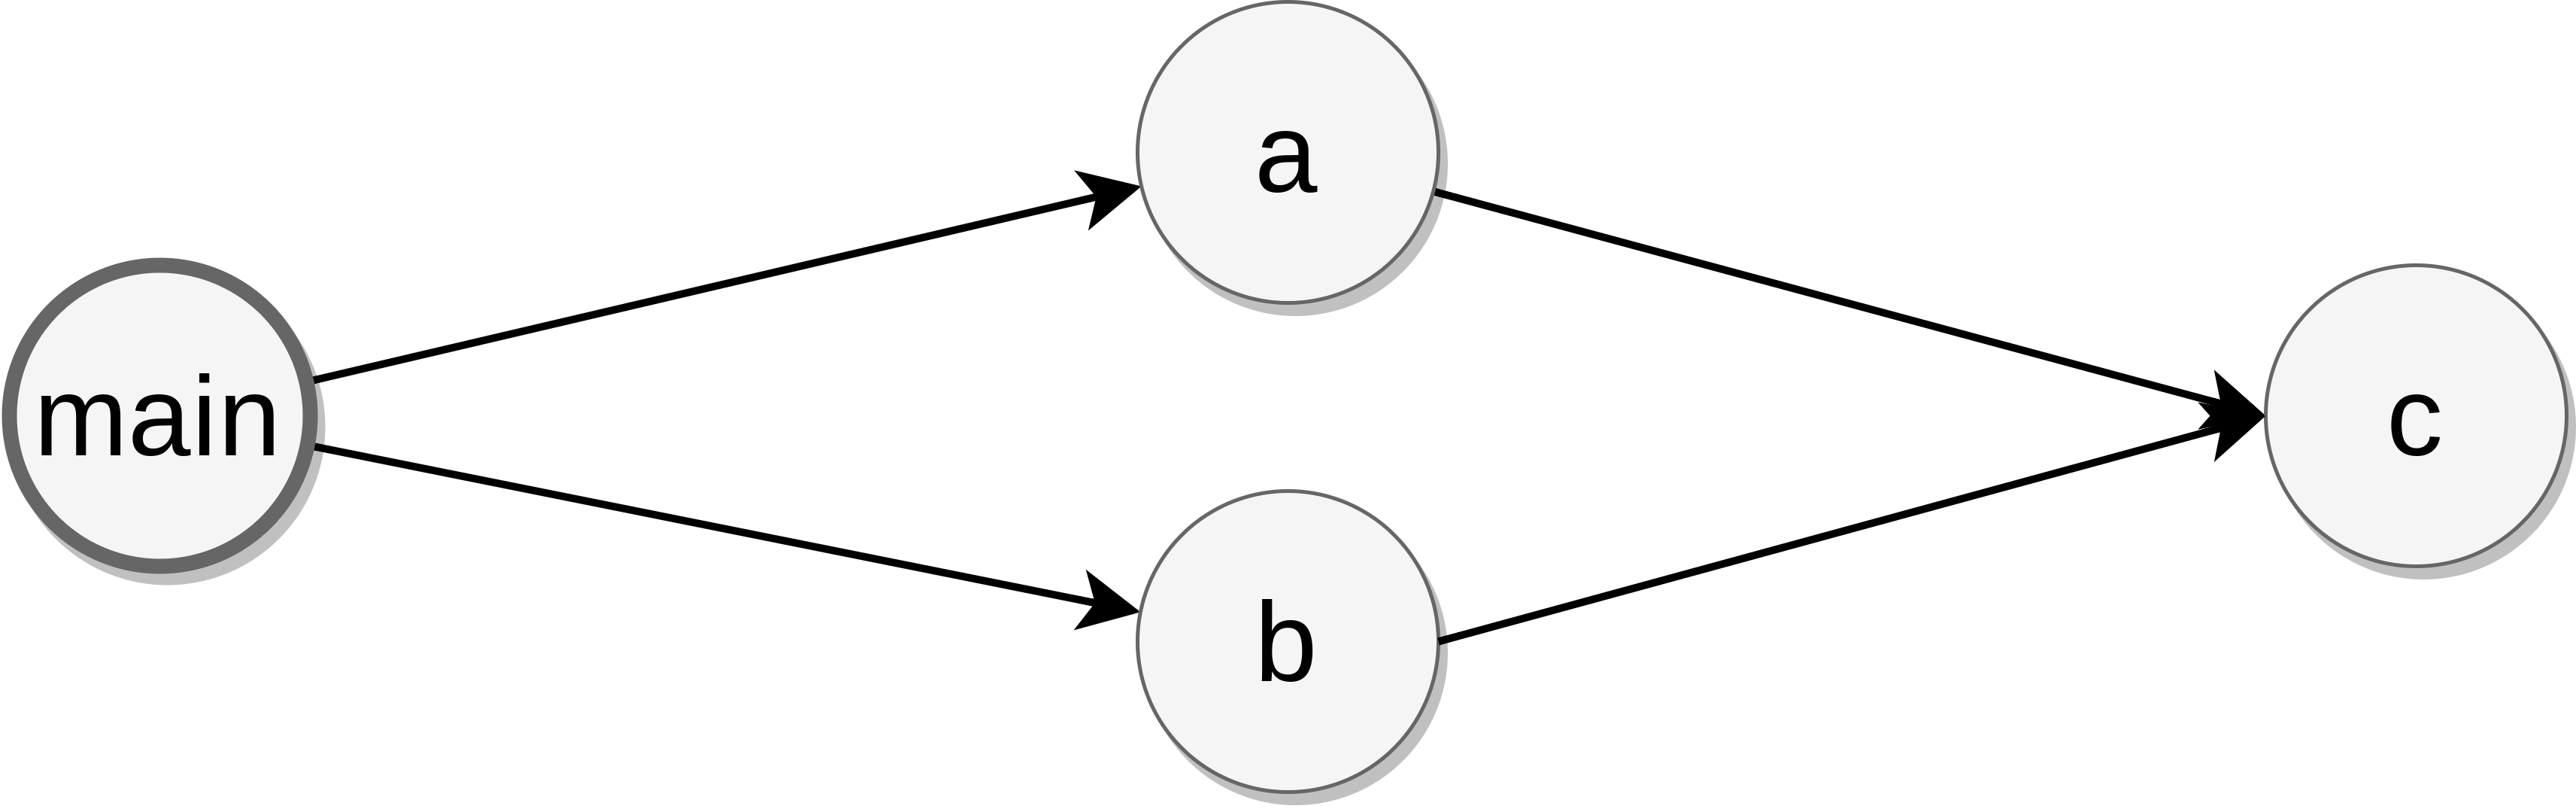
\includegraphics[width=0.4\textwidth]{./images/dependency-tree-Parallel.png}
    \caption{Dependency tree}
    \label{fig:dependency-tree-parallel}
\end{figure}

The formalization of this problem is as shown in Listing~\ref{lst:source-code-formalization}.

\begin{lstlisting}[caption=Source code formalization,label=lst:source-code-formalization,style=pddlStyle]
(:init
    (executed_instruction id0)

    (assignment_id assignmentA id1)
    (assignment_id assignmentB id2)
    (operation_id sumAB id3)
    (assignment_id assignmentC id4)
    
    (dependency_tree id0 id1)
    (dependency_tree id0 id2)
    (dependency_tree id1 id3)
    (dependency_tree id2 id3)
    (dependency_tree id3 id4)
)

(:goal (and
    (executed_assignment assignmentA)
    (executed_assignment assignmentB)
    (executed_binary_operation assignmentA assignmentB sumAB assignmentC)
    (executed_assignment assignmentC)
))
\end{lstlisting}

The main point of the Listing~\ref{lst:source-code-formalization} is on lines 9 and 10. In these lines, I define the \texttt{a} and \texttt{b} instructions as dependent only on the main instruction\footnote{The main instruction represents the starting point of the application.}. The STP output of this formalization is represented visually in Figure~\ref{fig:parallel-plan}.

\begin{figure}[h]
    \centering
    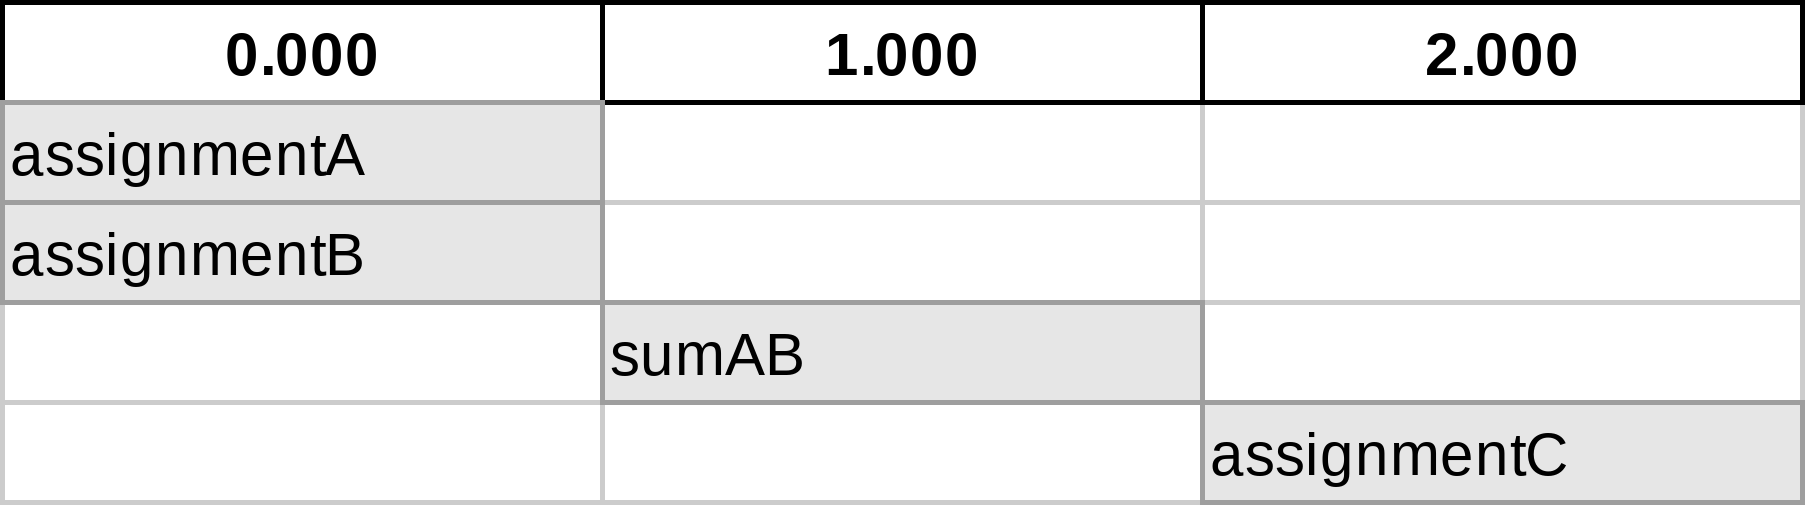
\includegraphics[width=0.4\textwidth]{./images/parallel-tasks-Parallel.png}
    \caption{STP parallel plan}
    \label{fig:parallel-plan}
\end{figure}

The Figure~\ref{fig:parallel-plan} shows that, as soon as the program starts, we can execute the \texttt{assignmentA} and \texttt{assignmentB} instructions at the same time. To execute the \texttt{sumAB} instruction, we must wait until the previous instructions are executed. Finally, to execute the \texttt{assignmentC} instruction, all previous instructions must be executed.

Imagining a source code similar to Listing~\ref{lst:source-code}, where the variable \texttt{b} is a result of the variable \texttt{a} plus 1, we would have a different dependency tree. Now, instead of line 10 in Listing~\ref{lst:source-code-formalization}, would be replaced by \texttt{(dependency\_tree\ id1\ id2)}, ensuring that variable \texttt{b} is assigned only after the variable \texttt{a}. The output of this second example is shown in Figure~\ref{fig:not-parallel-plan}.

\begin{figure}[h]
    \centering
    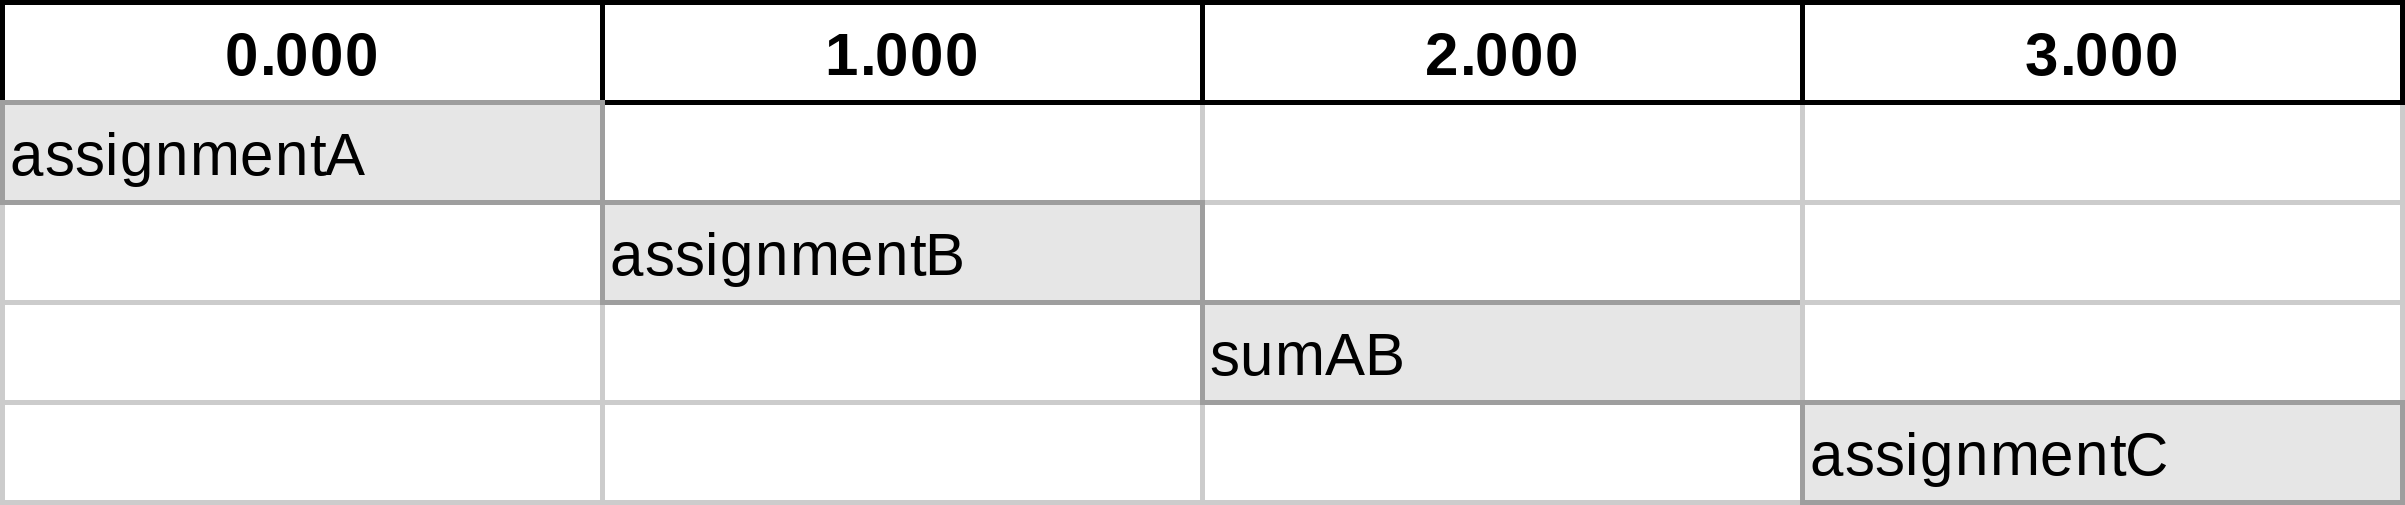
\includegraphics[width=0.43\textwidth]{./images/parallel-tasks-NotParallel.png}
    \caption{STP non-parallel plan}
    \label{fig:not-parallel-plan}
\end{figure}

\section{Conclusion}


\bibliographystyle{aaai}
\bibliography{references}

\end{document}